\documentclass[10pt]{article}
\usepackage[polish]{babel}
\usepackage[utf8]{inputenc}
\usepackage[T1]{fontenc}
\usepackage{graphicx}
\usepackage[export]{adjustbox}
\graphicspath{ {./images/} }
\usepackage{amsmath}
\usepackage{amsfonts}
\usepackage{amssymb}
\usepackage[version=4]{mhchem}
\usepackage{stmaryrd}

\title{ARKUSZ PRÓBNEJ MATURY Z OPERONEM MATEMATYKA \\
 POZIOM ROZSZERZONY }

\author{}
\date{}


\begin{document}
\maketitle
\section*{Czas pracy: 180 minut}
\section*{Instrukcja dla zdającego}
\begin{enumerate}
  \item Sprawdź, czy arkusz egzaminacyjny zawiera 12 stron (zadania 1.-16.). Ewentualny brak zgłoś przewodniczącemu zespołu nadzorującego egzamin.
  \item Rozwiązania zadań i odpowiedzi zapisz w miejscu na to przeznaczonym.
  \item W zadaniach zamkniętych (1.-5.) zaznacz jedną poprawną odpowiedź.
  \item W zadaniu kodowanym (6.) wpisz w tabelę wyniku trzy cyfry wymagane w poleceniu.
  \item W rozwiązaniach zadań otwartych (7.-16.) przedstaw tok rozumowania prowadzący do ostatecznego wyniku.
  \item Pisz czytelnie. Używaj długopisu/pióra tylko z czarnym tuszem/atramentem.
  \item Nie używaj korektora, a błędne zapisy wyraźnie przekreśl.
  \item Zapisy w brudnopisie nie będą oceniane.
  \item Obok numeru każdego zadania podana jest maksymalna liczba punktów możliwych do uzyskania.
  \item Możesz korzystać z zestawu wzorów matematycznych, cyrkla i linijki oraz kalkulatora.
\end{enumerate}

LISTOPAD 2019

Za rozwiązanie wszystkich zadań można otrzymać łącznie 50 punktów.

Życzymy powodzenia!

Wpisuje zdający przed rozpoczęciem pracy\\
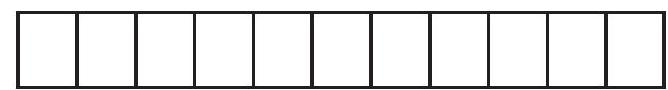
\includegraphics[max width=\textwidth, center]{2024_11_21_d15133c79177ee6989d3g-01}

PESEL ZDAJĄCEGO\\

\includegraphics[max width=\textwidth, center]{2024_11_21_d15133c79177ee6989d3g-01(1)}

KOD\\
ZDAJĄCEGO

Arkusz opracowany przez Wydawnictwo Pedagogiczne OPERON.\\
Kopiowanie w całości lub we fragmentach bez zgody wydawcy zabronione.

\section*{ZADANIA ZAMKNIĘTE}
W zadaniach 1.-5. wybierz i zaznacz jedną poprawną odpowiedź.

\section*{Zadanie 1. (0-1)}
Liczba \(\sqrt{11-6 \sqrt{2}}\) jest równa:\\
A. \(\sqrt{2}-3\)\\
B. \(3-\sqrt{2}\)\\
C. \(1-3 \sqrt{2}\)\\
D. \(3 \sqrt{2}-1\)

\section*{Zadanie 2. (0-1)}
Dziedziną funkcji \(f(x)=\log _{\frac{2 x-3}{x+3}}\left(x^{3}-x^{2}\right)\) jest:\\
A. \((-\infty,-3) \cup\left(\frac{3}{2},+\infty\right)\)\\
B. \((-\infty,-3) \cup(1,+\infty)\)\\
C. \((1,6) \cup(6,+\infty)\)\\
D. \(\left(\frac{3}{2}, 6\right) \cup(6,+\infty)\)

\section*{Zadanie 3. (0-1)}
Suma wszystkich współczynników wielomianu \(W(x)=\left(7 x^{3}-5 x^{2}-2 x+8\right)^{5}\) stojących przy nieparzystych potęgach zmiennej \(x\) wynosi:\\
A. \(2^{4}\left(2^{10}+1\right)\)\\
B. \(2^{4}\left(2^{10}-1\right)\)\\
C. \(2^{15}\)\\
D. \(-2^{5}\)

\section*{Zadanie 4. (0-1)}
Ile maksymalnie rozwiązań może mieć równanie \(|||x|-3|-2|=m\), gdzie \(m \in R\) ?\\
A. 2 rozwiązania\\
B. 4 rozwiązania\\
C. 8 rozwiązań\\
D. 16 rozwiązań

\section*{Zadanie 5. (0-1)}
Dany jest trapez równoramienny, w który wpisano okrąg. Odcinek łączący środki ramion trapezu ma długość 7 cm . Obwód tego trapezu jest równy:\\
A. 14 cm\\
B. 21 cm\\
C. 28 cm\\
D. 35 cm

\section*{BRUDNOPIS (nie podlega ocenie)}
\begin{center}

\includegraphics[max width=\textwidth]{2024_11_21_d15133c79177ee6989d3g-03}
\end{center}

\section*{ZADANIA OTWARTE}
\section*{Rozwiązania zadań 6.-16. należy zapisać w wyznaczonych miejscach pod treścią zadania.}
\section*{Zadanie 6. (0-2)}
Oblicz \(\lim _{x \rightarrow-2} \frac{x^{2}+7 x+10}{x^{3}+8}\).\\
Zakoduj cyfrę jedności i dwie kolejne cyfry po przecinku rozwinięcia dziesiętnego otrzymanego wyniku.\\
\(\square\)

\begin{center}
\begin{tabular}{|c|c|c|c|c|c|c|c|c|c|c|c|c|c|c|c|c|c|c|c|c|c|c|c|c|c|c|c|c|c|}
\hline
 &  &  &  &  &  &  &  &  &  &  &  &  &  &  &  &  &  &  &  &  &  &  &  &  &  &  &  &  &  \\
\hline
 &  &  &  &  &  &  &  &  &  &  &  &  &  &  &  &  &  &  &  &  &  &  &  &  &  &  &  &  &  \\
\hline
 &  &  &  &  &  &  &  &  &  &  &  &  &  &  &  &  &  &  &  &  &  &  &  &  &  &  &  &  &  \\
\hline
 &  &  &  &  &  &  &  &  &  &  &  &  &  &  &  &  &  &  &  &  &  &  &  &  &  &  &  &  &  \\
\hline
 &  &  &  &  &  &  &  &  &  &  &  &  &  &  &  &  &  &  &  &  &  &  &  &  &  &  &  &  &  \\
\hline
 &  &  &  &  &  &  &  &  &  &  &  &  &  &  &  &  &  &  &  &  &  &  &  &  &  &  &  &  &  \\
\hline
 &  &  &  &  &  &  &  &  &  &  &  &  &  &  &  &  &  &  &  &  &  &  &  &  &  &  &  &  &  \\
\hline
 &  &  &  &  &  &  &  &  &  &  &  &  &  &  &  &  &  &  &  &  &  &  &  &  &  &  &  &  &  \\
\hline
 &  &  &  &  &  &  &  &  &  &  &  &  &  &  &  &  &  &  &  &  &  &  &  &  &  &  &  &  &  \\
\hline
 &  &  &  &  &  &  &  &  &  &  &  &  &  &  &  &  &  &  &  &  &  &  &  &  &  &  &  &  &  \\
\hline
 &  &  &  &  &  &  &  &  &  &  &  &  &  &  &  &  &  &  &  &  &  &  &  &  &  &  &  &  &  \\
\hline
 &  &  &  &  &  &  &  &  &  &  &  &  &  &  &  &  &  &  &  &  &  &  &  &  &  &  &  &  &  \\
\hline
 &  &  & \(\square\) &  &  &  &  &  &  &  &  &  &  &  &  &  &  &  &  &  &  & 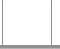
\includegraphics[max width=\textwidth]{2024_11_21_d15133c79177ee6989d3g-04(1)}
 & 
\includegraphics[max width=\textwidth]{2024_11_21_d15133c79177ee6989d3g-04(2)}
 &  & 
\includegraphics[max width=\textwidth]{2024_11_21_d15133c79177ee6989d3g-04}
 & 
\includegraphics[max width=\textwidth]{2024_11_21_d15133c79177ee6989d3g-04(3)}
 &  &  & 
\includegraphics[max width=\textwidth]{2024_11_21_d15133c79177ee6989d3g-04(4)}
 \\
\hline
\end{tabular}
\end{center}

\section*{Zadanie 7. (0-3)}
Wyznacz największą i najmniejszą wartość funkcji \(f(x)=\frac{x^{2}+8}{x+1}\) w przedziale \(\langle 0,3\rangle\).\\

\includegraphics[max width=\textwidth, center]{2024_11_21_d15133c79177ee6989d3g-04(5)}

Odpowiedź: \(\qquad\)

\section*{Zadanie 8. (0-3)}
Wykaż, że dla dowolnych liczb rzeczywistych \(x, y\) zachodzi nierówność \(2 x^{2}+5 y^{2}+10>6 x y+4 y\).

\begin{center}
\begin{tabular}{|c|c|c|c|c|c|c|c|c|c|c|c|c|c|c|c|c|c|c|c|c|c|c|c|c|c|c|c|c|c|}
\hline
 &  &  &  &  &  &  &  &  &  &  &  &  &  &  &  &  &  &  &  &  &  &  &  &  &  &  &  &  &  \\
\hline
 &  &  &  &  &  &  &  &  &  &  &  &  &  &  &  &  &  &  &  &  &  &  &  &  &  &  &  &  &  \\
\hline
 &  &  &  &  &  &  &  &  &  &  &  &  &  &  &  &  &  &  &  &  &  &  &  &  &  &  &  &  &  \\
\hline
 &  &  &  &  &  &  &  &  &  &  &  &  &  &  &  &  &  &  &  &  &  &  &  &  &  &  &  &  &  \\
\hline
 &  &  &  &  &  &  &  &  &  &  &  &  &  &  &  &  &  &  &  &  &  &  &  &  &  &  &  &  &  \\
\hline
 &  &  &  &  &  &  &  &  &  &  &  &  &  &  &  &  &  &  &  &  &  &  &  &  &  &  &  &  &  \\
\hline
 &  &  &  &  &  &  &  &  &  &  &  &  &  &  &  &  &  &  &  &  &  &  &  &  &  &  &  &  &  \\
\hline
 &  &  &  &  &  &  &  &  &  &  &  &  &  &  &  &  &  &  &  &  &  &  &  &  &  &  &  &  &  \\
\hline
. &  &  &  &  &  &  &  &  &  &  &  &  &  &  &  &  &  &  &  &  &  &  &  &  &  &  &  &  &  \\
\hline
 &  &  &  &  &  &  &  &  &  &  &  &  &  &  &  &  &  &  &  &  &  &  &  &  &  &  &  &  &  \\
\hline
- &  &  &  &  &  &  &  &  &  &  &  &  &  &  &  &  &  &  &  &  &  &  &  &  &  &  &  &  &  \\
\hline
- &  &  &  &  &  &  &  &  &  &  &  &  &  &  &  &  &  &  &  &  &  &  &  &  &  &  &  &  &  \\
\hline
 &  &  &  &  &  &  &  &  &  &  &  &  &  &  &  &  &  &  &  &  &  &  &  &  &  &  &  &  &  \\
\hline
 &  &  &  &  &  &  &  &  &  &  &  &  &  &  &  &  &  &  &  &  &  &  &  &  &  &  &  &  &  \\
\hline
 &  &  &  &  &  &  &  &  &  &  &  &  &  &  &  &  &  &  &  &  &  &  &  &  &  &  &  &  &  \\
\hline
\end{tabular}
\end{center}

\section*{Zadanie 9. (0-3)}
Dany jest trójkąt prostokątny o przyprostokątnych długości \(a \mathrm{i} b\), w którym kąt między środkową a wysokością wychodzącymi z wierzchołka kąta prostego ma miarę \(\alpha\). Wykaż, że \(\operatorname{tg} \alpha=\frac{\left|a^{2}-b^{2}\right|}{2 a b}\).

\begin{center}
\begin{tabular}{|c|c|c|c|c|c|c|c|c|c|c|c|c|c|c|c|c|c|c|c|c|c|c|c|c|c|c|c|c|}
\hline
 &  &  &  &  &  &  &  &  &  &  &  &  &  &  &  &  &  &  &  &  &  &  &  &  &  &  &  &  \\
\hline
 &  &  &  &  &  &  &  &  &  &  &  &  &  &  &  &  &  &  &  &  &  &  &  &  &  &  &  &  \\
\hline
 &  &  &  &  &  &  &  &  &  &  &  &  &  &  &  &  &  &  &  &  &  &  &  &  &  &  &  &  \\
\hline
 &  &  &  &  &  &  &  &  &  &  &  &  &  &  &  &  &  &  &  &  &  &  &  &  &  &  &  &  \\
\hline
 &  &  &  &  &  &  &  &  &  &  &  &  &  &  &  &  &  &  &  &  &  &  &  &  &  &  &  &  \\
\hline
 &  &  &  &  &  &  &  &  &  &  &  &  &  &  &  &  &  &  &  &  &  &  &  &  &  &  &  &  \\
\hline
 &  &  &  &  &  &  &  &  &  &  &  &  &  &  &  &  &  &  &  &  &  &  &  &  &  &  &  &  \\
\hline
 &  &  &  &  &  &  &  &  &  &  &  &  &  &  &  &  &  &  &  &  &  &  &  &  &  &  &  &  \\
\hline
 &  &  &  &  &  &  &  &  &  &  &  &  &  &  &  &  &  &  &  &  &  &  &  &  &  &  &  &  \\
\hline
 &  &  &  &  &  &  &  &  &  &  &  &  &  &  &  &  &  &  &  &  &  &  &  &  &  &  &  &  \\
\hline
 &  &  &  &  &  &  &  &  &  &  &  &  &  &  &  &  &  &  &  &  &  &  &  &  &  &  &  &  \\
\hline
- &  &  &  &  &  &  &  &  &  &  &  &  &  &  &  &  &  &  &  &  &  &  &  &  &  &  &  &  \\
\hline
 &  &  &  &  &  &  &  &  &  &  &  &  &  &  &  &  &  &  &  &  &  &  &  &  &  &  &  &  \\
\hline
- &  &  &  &  &  &  &  &  &  &  &  &  &  &  &  &  &  &  &  &  &  &  &  &  &  &  &  &  \\
\hline
 &  &  &  &  &  &  &  &  &  &  &  &  &  &  &  &  &  &  &  &  &  &  &  &  &  &  &  &  \\
\hline
 &  &  &  &  &  &  &  &  &  &  &  &  &  &  &  &  &  &  &  &  &  &  &  &  &  &  &  &  \\
\hline
 &  &  &  &  &  &  &  &  &  &  &  &  &  &  &  &  &  &  &  &  &  &  &  &  &  &  &  &  \\
\hline
\end{tabular}
\end{center}

\section*{Zadanie 10. (0-4)}
Rozwiąż równanie \(\cos 3 x+\sin 7 x=0 \mathrm{w}\) przedziale \(\langle 0, \pi\rangle\).

\begin{center}
\begin{tabular}{|c|c|c|c|c|c|c|c|c|c|c|c|c|c|c|c|c|c|c|c|c|c|c|c|c|c|c|c|c|c|}
\hline
 &  &  &  &  &  &  &  &  &  &  &  &  &  &  &  &  &  &  &  &  &  &  &  &  &  &  &  &  &  \\
\hline
 &  &  &  &  &  &  &  &  &  &  &  &  &  &  &  &  &  &  &  &  &  &  &  &  &  &  &  &  &  \\
\hline
 &  &  &  &  &  &  &  &  &  &  &  &  &  &  &  &  &  &  &  &  &  &  &  &  &  &  &  &  &  \\
\hline
 &  &  &  &  &  &  &  &  &  &  &  &  &  &  &  &  &  &  &  &  &  &  &  &  &  &  &  &  &  \\
\hline
 &  &  &  &  &  &  &  &  &  &  &  &  &  &  &  &  &  &  &  &  &  &  &  &  &  &  &  &  &  \\
\hline
 &  &  &  &  &  &  &  &  &  &  &  &  &  &  &  &  &  &  &  &  &  &  &  &  &  &  &  &  &  \\
\hline
 &  &  &  &  &  &  &  &  &  &  &  &  &  &  &  &  &  &  &  &  &  &  &  &  &  &  &  &  &  \\
\hline
 &  &  &  &  &  &  &  &  &  &  &  &  &  &  &  &  &  &  &  &  &  &  &  &  &  &  &  &  &  \\
\hline
 &  &  &  &  &  &  &  &  &  &  &  &  &  &  &  &  &  &  &  &  &  &  &  &  &  &  &  &  &  \\
\hline
 &  &  &  &  &  &  &  &  &  &  &  &  &  &  &  &  &  &  &  &  &  &  &  &  &  &  &  &  &  \\
\hline
 &  &  &  &  &  &  &  &  &  &  &  &  &  &  &  &  &  &  &  &  &  &  &  &  &  &  &  &  &  \\
\hline
 &  &  &  &  &  &  &  &  &  &  &  &  &  &  &  &  &  &  &  &  &  &  &  &  &  &  &  &  &  \\
\hline
 &  &  &  &  &  &  &  &  &  &  &  &  &  &  &  &  &  &  &  &  &  &  &  &  &  &  &  &  &  \\
\hline
 &  &  &  &  &  &  &  &  &  &  &  &  &  &  &  &  &  &  &  &  &  &  &  &  &  &  &  &  &  \\
\hline
 &  &  &  &  &  &  &  &  &  &  &  &  &  &  &  &  &  &  &  &  &  &  &  &  &  &  &  &  &  \\
\hline
 &  &  &  &  &  &  &  &  &  &  &  &  &  &  &  &  &  &  &  &  &  &  &  &  &  &  &  &  &  \\
\hline
\end{tabular}
\end{center}

Odpowiedź:

\section*{Zadanie 11. (0-4)}
W urnie umieszczono 4 kule białe i 8 kul czarnych. Losujemy jedną kulę. Jeżeli będzie biała, to wrzucamy ją z powrotem do urny i dorzucamy do niej jeszcze dwie białe kule. Jeżeli będzie czarna, to zatrzymujemy ją i dorzucamy dwie zielone kule do urny. Następnie losujemy z urny jednocześnie dwie kule. Oblicz prawdopodobieństwo zdarzenia, że obie z wylosowanych za drugim razem kul są białe.\\

\includegraphics[max width=\textwidth, center]{2024_11_21_d15133c79177ee6989d3g-06}

Odpowiedź: \(\qquad\)

\section*{Zadanie 12. (0-4)}
Graniastosłup prawidłowy czworokątny o krawędzi podstawy \(a\) i dwa razy krótszej wysokości przecięto płaszczyzną przechodzącą przez przekątną podstawy i nachyloną do płaszczyzny podstawy pod kątem \(60^{\circ}\). Zaznacz ten kąt na rysunku oraz oblicz pole otrzymanego przekroju, wynik przedstaw w najprostszej postaci.\\

\includegraphics[max width=\textwidth, center]{2024_11_21_d15133c79177ee6989d3g-07}

Odpowiedź:

\section*{Zadanie 13. (0-6)}
Wyznacz wartość parametru \(m\), dla którego równanie \(\left(m^{2}+m-3\right) x^{2}+(2 m-1) x+2=0\) ma dwa rozwiązania dodatnie takie, że jedno z nich jest dwa razy większe od drugiego.\\

\includegraphics[max width=\textwidth, center]{2024_11_21_d15133c79177ee6989d3g-08}

Odpowiedź:\\
8

\section*{Zadanie 14. (0-4)}
Wyznacz równanie okręgu opisanego na trójkącie, k tórego boki zawierają się w prostych o równaniach \(x+6 y-12=0 ; x+y-7=0\) oraz \(x-4 y+18=0\).\\

\includegraphics[max width=\textwidth, center]{2024_11_21_d15133c79177ee6989d3g-09}

Odpowiedź: \(\qquad\)

\section*{Zadanie 15. (0-5)}
Rozwiąż nierówność \(\frac{1}{x-3}+\frac{1}{(x-3)^{2}}+\frac{1}{(x-3)^{3}}+\cdots \geq 2-x\), gdzie lewa strona nierówności jest szeregiem geometrycznym zbieżnym. Podaj odpowiednie założenia.\\

\includegraphics[max width=\textwidth, center]{2024_11_21_d15133c79177ee6989d3g-10}

Odpowiedź: \(\qquad\)\\
10

\section*{Zadanie 16. (0-7)}
Powierzchnia całkowita graniastosłupa prawidłowego sześciokątnego jest równa \(S \sqrt{3}\). Wyznacz największą z możliwych objętość tego graniastosłupa, wynik zapisz w najprostszej postaci.\\

\includegraphics[max width=\textwidth, center]{2024_11_21_d15133c79177ee6989d3g-11}

Odpowiedź: \(\qquad\)

\section*{BRUDNOPIS (nie podlega ocenie)}
\begin{center}

\includegraphics[max width=\textwidth]{2024_11_21_d15133c79177ee6989d3g-12}
\end{center}


\end{document}